\documentclass[10pt,conference]{IEEEtran}
\usepackage[T1]{fontenc}
\usepackage{graphicx}
\usepackage{booktabs}
\usepackage{tabularx}
\usepackage{multirow}
\usepackage{microtype}
\usepackage{xcolor}
\usepackage{url}
\newcolumntype{Y}{>{\raggedright\arraybackslash}X}
\title{Cross-Session Tool-Trajectory Detection in LLM Agents: A Replicated Study of Detection--False-Alarm Trade-offs}
\author{\IEEEauthorblockN{Xiangyi Li}\IEEEauthorblockA{Independent Researcher\\Contact information to be supplied for submission}}
\begin{document}
\maketitle
\begin{abstract}
LLM agents turn language-model outputs into sequences of tool calls, so a harmful objective may be expressed across several sessions rather than in one isolated prompt. This paper re-evaluates a cross-session trajectory detector under a frozen, API-executed protocol. A trajectory-only candidate was selected during development (R1--R3), then locked before two independent confirmation runs (R4--R5) with new prompt wording, operands, and long normal controls. On successful attack objectives, the candidate recalled $42.8\%\pm1.3\%$ while producing $0.25\%\pm0.35\%$ false positives across runs; under exact output-length matching, recall fell to $22.2\%$--$25.7\%$. A diagnostic ablation shows that transition/frequency signals are indispensable, whereas the proposed cross-session graph supplies little incremental benefit in this setting. A post-hoc removal of cumulative scoring performs much better, but is explicitly reported as exploratory rather than confirmatory. An official AgentShield implementation achieves perfect recall in separate honeytool-augmented executions, so no paired superiority claim is made. The contribution is therefore a reproducible measurement protocol and a calibrated account of what this detector does and does not establish, rather than a production-readiness claim.
\end{abstract}
\begin{IEEEkeywords}
LLM agents, agent security, tool trajectories, cross-session detection, reproducible evaluation
\end{IEEEkeywords}

\section{Introduction}
Tool-using LLM agents can browse, retrieve, transact, and communicate. Their security-relevant behavior is consequently a trajectory: an apparently benign call may become harmful only in the context of earlier calls, repeated transitions, or accumulated intent. This motivates cross-session behavioral monitoring, but it also creates a demanding evaluation problem. A detector can appear effective when attack traces are longer, when a threshold is selected on the test set, or when a protected baseline changes the executed environment.

This manuscript replaces a performance-oriented interpretation of an earlier prototype with a frozen, independent evaluation. Its central research question is narrow: \emph{what detection--false-alarm trade-off does a trajectory score provide after candidate selection is separated from confirmation?} The answer is mixed. The locked candidate detects a material fraction of attacks at a low false-positive rate, but it misses most successful objectives and does not justify a deployment or superiority claim.

\section{Detector and Frozen Protocol}
The candidate maintains decayed transition counts and benign frequency estimates for tool-call trajectories. It scores a session using transition and frequency deviations, then accumulates evidence across the trajectory. Parameter-level rules, tool-combination rules, and a claimed graph-structure component are excluded from the locked candidate because they did not survive development diagnostics. The alarm threshold is fixed before test evaluation as the smallest value above the maximum score among 100 benign validation trajectories.

\begin{figure*}[t]
\centering
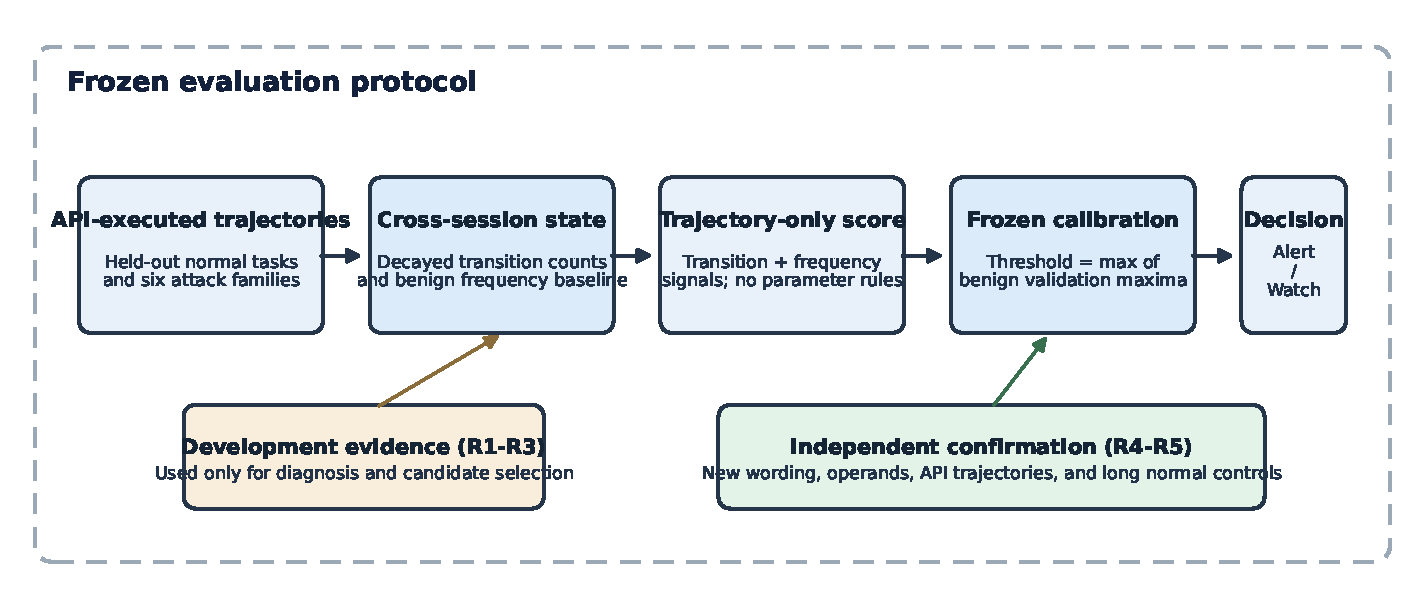
\includegraphics[width=.96\textwidth]{assets/figure1_protocol.pdf}
\caption{Evaluation architecture. R1--R3 are development-only evidence. The candidate and calibration rule are frozen before R4--R5, which use new wording, operands, API-executed trajectories, and long normal controls.}
\label{fig:protocol}
\end{figure*}

\begin{table}[t]
\caption{Separation of development and independent confirmation. Counts are per R4/R5 run.}
\label{tab:protocol}
\centering\footnotesize
\begin{tabularx}{\columnwidth}{@{}lYY@{}}
\toprule
Item & Development (R1--R3) & Confirmation (R4--R5)\\
\midrule
Role & candidate selection and diagnosis & frozen evaluation\\
Normal calibration & used during development & 200 (100 short, 100 long)\\
Validation normal & -- & 100\\
Test normal & -- & 200\\
Attack groups & development templates & 240; six held-out families\\
Execution & API traces & API traces; new operands and wording\\
\bottomrule
\end{tabularx}
\end{table}

\section{Experimental Design}
Each independent run includes 240 attack groups, 200 normal test groups, 100 validation-normal groups, and 200 calibration-normal groups. Attack groups span indirect injection, tool exfiltration, transaction cover, privilege escalation, and related multi-step patterns. The reported ``successful-attack recall'' conditions on objectives that actually succeeded (160 in each run); all-attempt detection includes every attack attempt. We use nonparametric bootstrap intervals over groups for within-run rates. R4/R5 are independent confirmation repetitions, not hyperparameter searches.

The main comparison is intentionally limited. The official AgentShield implementation is run unchanged behind a local adapter, but its honeytools and honeytokens alter agent behavior. It therefore receives its own defended executions, rather than paired replays of identical traces. Its values are descriptive reference measurements, not inputs to paired tests or claims of statistical superiority.

\section{Independent Confirmation Results}
Table~\ref{tab:main} reports the prespecified candidate. The low aggregate false-positive rate is real but uncertain at this sample size. More importantly, successful-attack recall is only $41.9\%$ in R4 and $43.8\%$ in R5. Exact length matching further reduces recall, ruling out the interpretation that the main result controls fully for attack-trace length. Figure~\ref{fig:ecdf} exposes the overlap directly: a high validation-maximum threshold protects normal traffic but leaves many attack groups below the alarm boundary.

\begin{table}[t]
\caption{Frozen candidate on independent confirmation. Bootstrap CIs are 95\% intervals.}
\label{tab:main}
\centering\footnotesize
\begin{tabular}{@{}lcc@{}}
\toprule
Metric & R4 & R5\\
\midrule
All-attempt detection & 28.3\% [22.5, 34.2] & 29.6\% [23.8, 35.4]\\
Successful-attack recall & 41.9\% [34.4, 49.4] & 43.8\% [36.3, 51.9]\\
False-positive rate & 0.0\% [0.0, 0.0] & 0.5\% [0.0, 1.5]\\
Length-matched detection & 22.2\% [14.5, 29.9] & 25.7\% [17.7, 33.6]\\
\bottomrule
\end{tabular}
\end{table}

\begin{figure}[t]
\centering
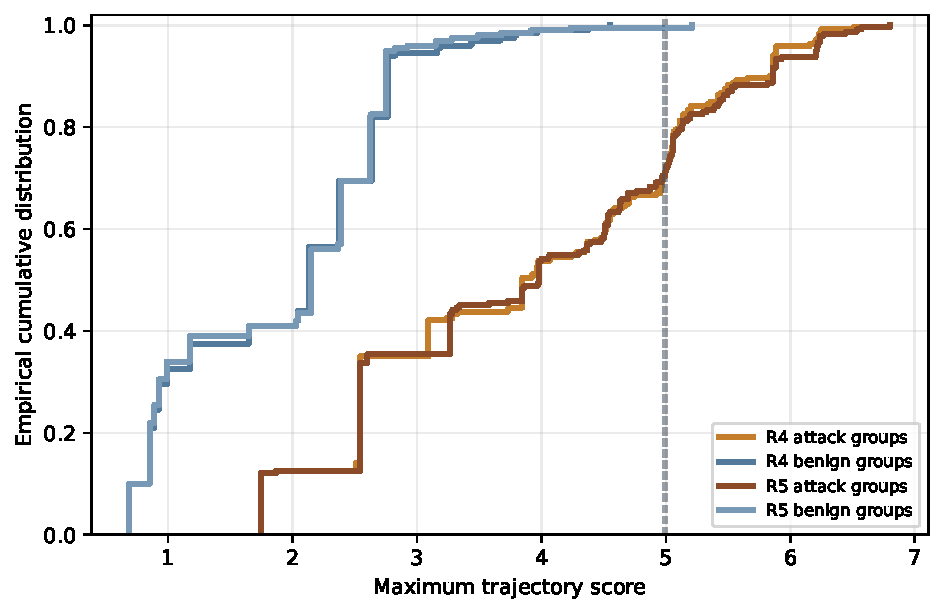
\includegraphics[width=\columnwidth]{assets/figure2_score_ecdf.pdf}
\caption{Empirical CDFs of maximum trajectory score. Dashed lines are frozen validation-maximum thresholds; attack and benign score distributions overlap substantially.}
\label{fig:ecdf}
\end{figure}

\begin{figure}[t]
\centering
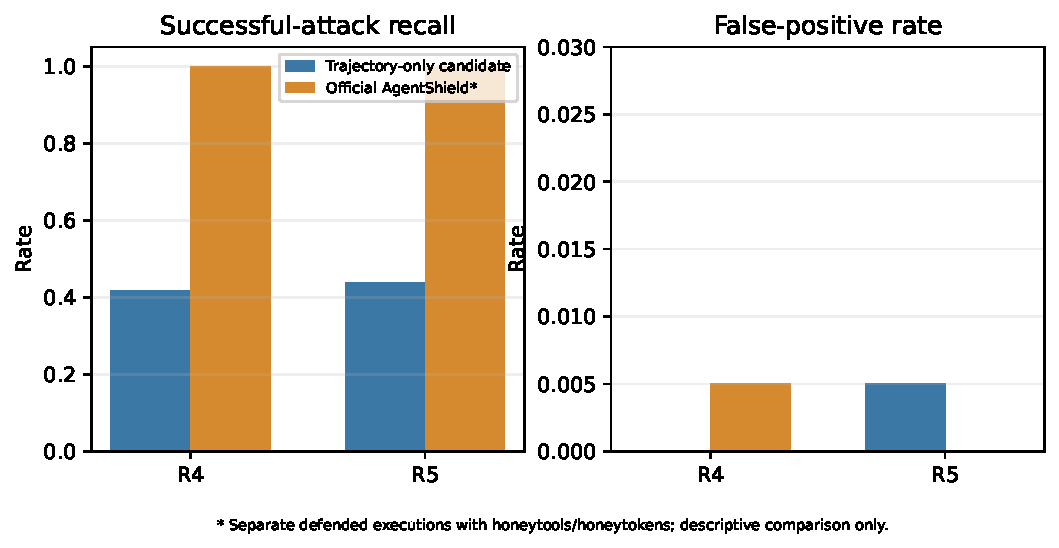
\includegraphics[width=\columnwidth]{assets/figure3_confirmation.pdf}
\caption{Independent confirmation versus the official AgentShield baseline. AgentShield values use separate honeytool/honeytoken-protected executions and are descriptive only.}
\label{fig:baseline}
\end{figure}

\section{Mechanism Diagnostics and Failure Analysis}
The most important mechanistic finding is negative. Removing the cross-session feature changes all-attempt detection by less than half a percentage point. In contrast, removing transition/frequency signals eliminates detection under the same calibration rule. Removing cumulative scoring produces $95\%$ and $100\%$ all-attempt detection in R4/R5. Since this latter ablation was performed after examining confirmation data, it is a hypothesis for R6/R7 replication, not a replacement for the frozen primary result.

\begin{table}[t]
\caption{Post-confirmation exploratory ablation. Values are all-attempt detection; they must not be interpreted as confirmatory model selection.}
\label{tab:ablation}
\centering\footnotesize
\begin{tabular}{@{}lcc@{}}
\toprule
Variant & R4 & R5\\
\midrule
Frozen trajectory-only candidate & 28.3\% & 29.6\%\\
No cross-session component & 27.9\% & 29.2\%\\
No transition/frequency signal & 0.0\% & 0.0\%\\
No cumulative scoring (exploratory) & 95.0\% & 100.0\%\\
\bottomrule
\end{tabular}
\end{table}

\begin{figure}[t]
\centering
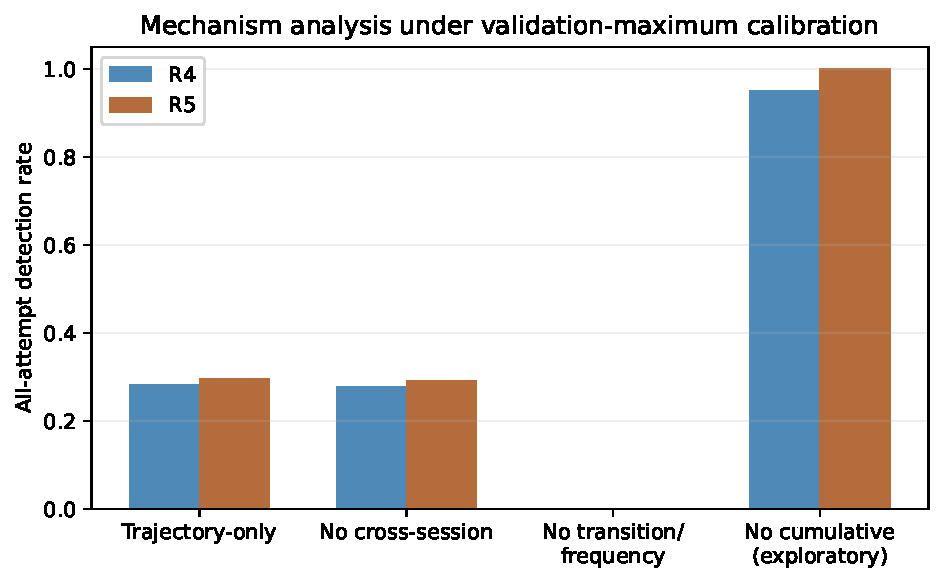
\includegraphics[width=\columnwidth]{assets/figure4_ablation.pdf}
\caption{Exploratory mechanism analysis at the validation-maximum calibration. The striking no-cumulative result requires a fresh preregistered replication before it can support a method claim.}
\label{fig:ablation}
\end{figure}

Across R4/R5, 183 successful objectives were missed. Indirect injection accounted for 80, tool exfiltration for 47, transaction cover for 48, and privilege escalation for 8. These errors indicate a concrete weakness: the current score detects unusual transitions but can miss a harmful objective whose individual calls resemble normal trajectories.

\section{Threats to Validity and Responsible Scope}
This study evaluates one API-accessible model and a banking-style tool sandbox; it does not establish cross-model generalization, real-world coverage, or robustness to adaptive attackers. Attack templates and normal tasks may not represent natural deployment traffic. The aggregate false-positive estimate has wide uncertainty because only 400 independent test-normal groups are observed. Long-control matching reduces, but does not eliminate, confounding from trace length. Finally, the environment-altering AgentShield comparison cannot identify a paired causal advantage.

Accordingly, this work should be read as an auditable benchmark and a negative/diagnostic result. Before deployment, future work must preregister R6/R7 for the non-cumulative hypothesis, add independently implemented official baselines where available, evaluate multiple models and tool domains, and test adaptive attacks without reusing selection data.

\section{Conclusion}
Cross-session trajectory monitoring is a worthwhile security direction, but the present candidate is not a production-ready detector. Independent confirmation shows low false positives alongside limited attack recall, negligible measured value from the cross-session component, and substantial failure modes. The revised claim is deliberately narrower: frozen evaluation and transparent diagnostics are necessary to distinguish promising trajectory signals from an overstated safety result.

\begin{thebibliography}{00}
\bibitem{agentshield} Y. H. Rassul and T. A. Rashid, ``AgentShield: Deception-based Compromise Detection for Tool-using LLM Agents,'' arXiv:2605.11026, 2026.
\bibitem{fragbench} A. Mehta et al., ``FragBench: Cross-Session Attacks Hidden in Benign-Looking Fragments,'' arXiv:2605.11029, 2026.
\end{thebibliography}
\end{document}
